%%%%%%%%%%%%%%%%%%%%%%%%%%%%%%%%%%%%%%%%%%%%%%%%%%%%%%%%%%%%%%%%%%%%%%%%%%%

\documentclass{standalone}

\usepackage{amsmath}
\usepackage{mathptmx}
\usepackage{pgfplots}
\usetikzlibrary{external}
\tikzexternalize{yeast}
\pgfplotsset{compat=1.15}

%% IEEE uses Times Roman font, so we'll default to Times.
%% These three commands make up the entire times.sty package.
\renewcommand{\rmdefault}{ptm}
\renewcommand{\ttdefault}{pcr}
\normalfont\selectfont

\begin{document}

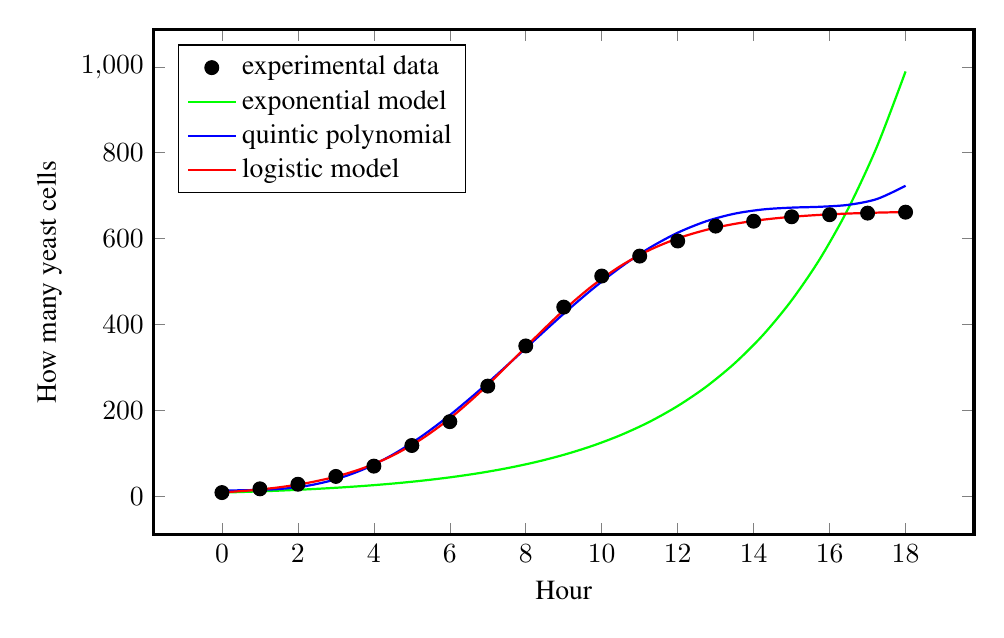
\begin{tikzpicture}
\tikzset{%%
  every mark/.append style={scale=1.0},%%
  scale=1.0%%
}
\pgfplotsset{%%
  every axis/.append style={font=\normalsize}%%
}
%%
\begin{axis}[%%
  axis line style=very thick,%%
  dotStyle/.style={mark size=2.5,black,mark color=black,mark=*,only marks},%%
  enlargelimits=true,%%
  height=8cm,%%
  legend cell align=left,%%
  legend pos=north west,%%
  plotStyle/.style={%%
    domain=0:18,%%
    mark=none,%%
    smooth,%%
    thick%%
  },%%
  width=12cm,%%
  %% x axis
  xlabel={\normalsize Hour},%%
  %% y axis
  ylabel={\normalsize How many yeast cells},%%
  scaled y ticks=false,%%
  y tick label style=/pgf/number format/fixed%%
]
%%
%%
\addplot[dotStyle] coordinates {
  (0, 9.6)
  (1, 18.3)
  (2, 29)
  (3, 47.2)
  (4, 71.1)
  (5, 119.1)
  (6, 174.6)
  (7, 257.3)
  (8, 350.7)
  (9, 441)
  (10, 513.3)
  (11, 559.7)
  (12, 594.8)
  (13, 629.4)
  (14, 640.8)
  (15, 651.1)
  (16, 655.9)
  (17, 659.6)
  (18, 661.8)
};
\addlegendentry{experimental data}
%%
%%
%% The exponential model.
\addplot+ [plotStyle,green]
{9.6*(1.2937^x)};
\addlegendentry{exponential model}
%%
%%
%% The quintic polynomial.
\addplot+ [plotStyle,blue]
{0.0052*x^5 - 0.2069*x^4 + 2.3331*x^3 - 3.2478*x^2 + 2.6845*x + 14.2567};
\addlegendentry{quintic polynomial}
%%
%%
%% The logistic model.
\addplot+ [plotStyle,red]
{665 / (1 + exp(4.1896 - 0.5355*x))};
\addlegendentry{logistic model}
\end{axis}
\end{tikzpicture}

\end{document}
